\documentclass[tikz]{standalone}
\usetikzlibrary{decorations.pathreplacing}

\begin{document}
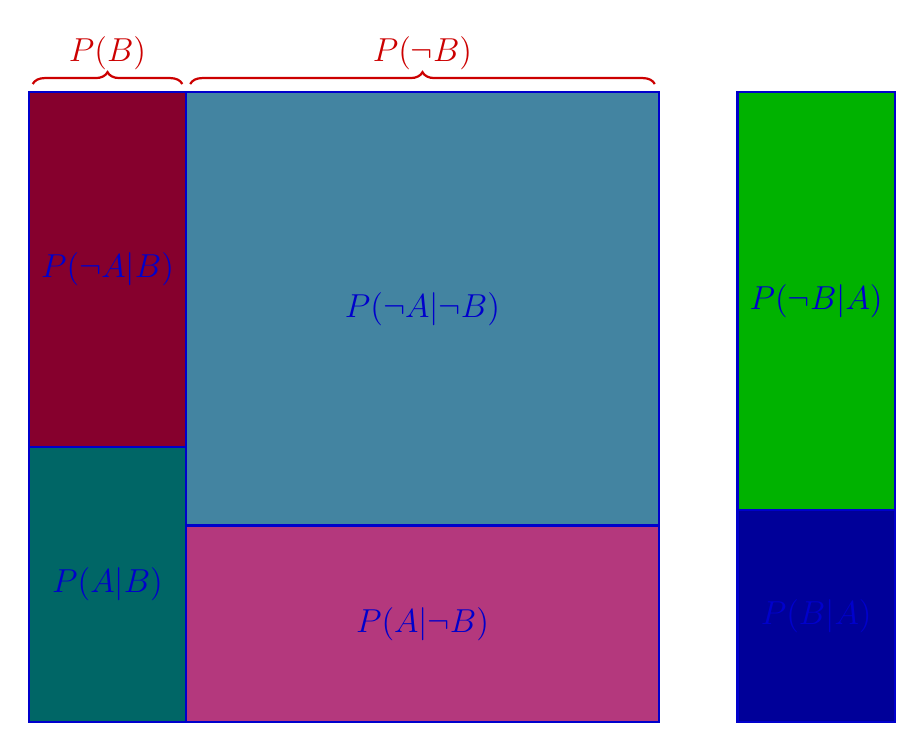
\begin{tikzpicture}[thick, font=\large, draw=blue!80!black, text=blue!80!black]

  % Left vertical rectangles (conditional probabilities)
  \draw[fill=teal!80!black] (0,0) rectangle (2,3.5) node[midway] (pAB) {$P(A|B)$};
  \draw[fill=purple!70!black] (0,3.5) rectangle (2,8) node[midway] (pAnB) {$P(\neg A|B)$};

  % Right horizontal rectangles (conditional probabilities)
  \draw[fill=magenta!70!black] (2,0) rectangle (8,2.5) node[midway] (pBnA) {$P(A|\neg B)$};
  \draw[fill=cyan!60!black] (2,2.5) rectangle (8,8) node[midway] (pAnBnA) {$P(\neg A|\neg B)$};

  % Top braces for prior probabilities
  \draw[red!80!black, decorate, decoration={brace, amplitude=1ex, raise=3pt}] (0.05,8) -- (1.95,8) node[midway, above=1ex, text=red!80!black] {$P(B)$};
  \draw[red!80!black, decorate, decoration={brace, amplitude=1ex, raise=3pt}] (2.05,8) -- (7.95,8) node[midway, above=1ex, text=red!80!black] {$P(\neg B)$};

  % Right vertical rectangles (posterior probabilities)
  \draw[fill=blue!60!black] (9,0) rectangle (11,2.7) node[midway] (pBA) {$P(B|A)$};
  \draw[fill=green!70!black] (9,2.7) rectangle (11,8) node[midway] (pnBA) {$P(\neg B|A)$};

\end{tikzpicture}
\end{document}